\documentclass[tikz,border=7pt]{standalone}
\usepackage{amsmath}
\usetikzlibrary{arrows.meta,calc,positioning,decorations.pathreplacing}
\def\figcellw{0.90cm}\def\figcellh{0.36cm}
% Shared palette and TikZ styles for the information-flow figures.
%
% Each figure sets its cell size before loading this file:
%   \def\figcellw{0.80cm}\def\figcellh{0.36cm}
%   % Shared palette and TikZ styles for the information-flow figures.
%
% Each figure sets its cell size before loading this file:
%   \def\figcellw{0.80cm}\def\figcellh{0.36cm}
%   % Shared palette and TikZ styles for the information-flow figures.
%
% Each figure sets its cell size before loading this file:
%   \def\figcellw{0.80cm}\def\figcellh{0.36cm}
%   \input{figure_style}
\providecommand{\figcellw}{0.80cm}
\providecommand{\figcellh}{0.36cm}

% ------------------------------------------------------------
% Palette
% ------------------------------------------------------------
\definecolor{frameblue}{RGB}{42,66,167}
\definecolor{headerfill}{RGB}{238,242,252}
\definecolor{activefill}{RGB}{210,235,250}
\definecolor{activedraw}{RGB}{0,137,225}
\definecolor{ghostfill}{RGB}{222,228,236}
\definecolor{ghostdraw}{RGB}{145,154,168}
\definecolor{depthfill}{RGB}{249,221,187}
\definecolor{depthdraw}{RGB}{216,108,19}
\definecolor{tempfill}{RGB}{229,210,252}
\definecolor{tempdraw}{RGB}{119,45,205}

% ------------------------------------------------------------
% Styles
% ------------------------------------------------------------
\tikzset{
  % Frames and headers
  panel/.style={draw=frameblue, rounded corners=4pt, line width=0.9pt},
  header/.style={draw=frameblue, fill=headerfill, rounded corners=4pt, line width=0.9pt},
  sideheader/.style={header},
  descbox/.style={draw=frameblue!55, fill=white, rounded corners=2.5pt, line width=0.6pt,
    inner sep=2pt, align=center, font=\footnotesize,
    execute at begin node={\hyphenpenalty=10000\exhyphenpenalty=10000\relax}},
  divider/.style={draw=frameblue, dashed, line width=0.8pt},
  % Layer and block cells
  cell/.style={rounded corners=2pt, minimum width=\figcellw, minimum height=\figcellh, inner sep=0pt},
  active/.style={cell, draw=activedraw, fill=activefill, line width=0.82pt},
  ghost/.style={cell, draw=ghostdraw, fill=ghostfill, fill opacity=0.42, draw opacity=0.58, line width=0.72pt},
  depthmark/.style={cell, draw=depthdraw, fill=depthfill, line width=0.95pt},
  tempmark/.style={cell, draw=tempdraw, fill=tempfill, line width=0.95pt},
  depthcell/.style={depthmark},
  tempcell/.style={tempmark},
  ghostdepth/.style={cell, draw=depthdraw, fill=depthfill, fill opacity=0.28, draw opacity=0.55, line width=0.90pt},
  ghosttemp/.style={cell, draw=tempdraw, fill=tempfill, fill opacity=0.28, draw opacity=0.55, line width=0.90pt},
  notrun/.style={cell, draw=ghostdraw, dashed, draw opacity=0.7, line width=0.6pt},
  stateT/.style={cell, draw=tempdraw, fill=tempfill, inner sep=1pt, line width=0.9pt, font=\footnotesize},
  stateD/.style={cell, draw=depthdraw, fill=depthfill, inner sep=1pt, line width=0.9pt, font=\footnotesize},
  % State injection points
  injectD/.style={circle, draw=depthdraw, fill=depthfill, minimum size=3.6mm,
    inner sep=0pt, line width=0.85pt, font=\bfseries\scriptsize},
  injectT/.style={circle, draw=tempdraw, fill=tempfill, minimum size=3.6mm,
    inner sep=0pt, line width=0.85pt, font=\bfseries\scriptsize},
  % Arrows
  flow/.style={-{Latex[length=1.8mm]}, draw=black, line width=0.82pt},
  injflow/.style={-{Latex[length=1.25mm]}, draw=black, line width=0.82pt},
  ghostflow/.style={-{Latex[length=1.5mm]}, draw=black!38, line width=0.58pt},
  dread/.style={-{Latex[length=1.9mm]}, draw=depthdraw, dashed, line width=0.95pt},
  tread/.style={-{Latex[length=1.9mm]}, draw=tempdraw, dashed, line width=0.95pt},
  % Labels
  brace label/.style={midway, xshift=-0.86cm, align=right, text width=1.32cm, font=\footnotesize},
  rlabel/.style={anchor=east, font=\footnotesize, align=right, text width=1.65cm},
  stage/.style={anchor=east, font=\footnotesize, align=right, text width=1.8cm},
  tinylabel/.style={font=\footnotesize, align=center},
  legendtext/.style={anchor=west, font=\footnotesize},
}

\providecommand{\figcellw}{0.80cm}
\providecommand{\figcellh}{0.36cm}

% ------------------------------------------------------------
% Palette
% ------------------------------------------------------------
\definecolor{frameblue}{RGB}{42,66,167}
\definecolor{headerfill}{RGB}{238,242,252}
\definecolor{activefill}{RGB}{210,235,250}
\definecolor{activedraw}{RGB}{0,137,225}
\definecolor{ghostfill}{RGB}{222,228,236}
\definecolor{ghostdraw}{RGB}{145,154,168}
\definecolor{depthfill}{RGB}{249,221,187}
\definecolor{depthdraw}{RGB}{216,108,19}
\definecolor{tempfill}{RGB}{229,210,252}
\definecolor{tempdraw}{RGB}{119,45,205}

% ------------------------------------------------------------
% Styles
% ------------------------------------------------------------
\tikzset{
  % Frames and headers
  panel/.style={draw=frameblue, rounded corners=4pt, line width=0.9pt},
  header/.style={draw=frameblue, fill=headerfill, rounded corners=4pt, line width=0.9pt},
  sideheader/.style={header},
  descbox/.style={draw=frameblue!55, fill=white, rounded corners=2.5pt, line width=0.6pt,
    inner sep=2pt, align=center, font=\footnotesize,
    execute at begin node={\hyphenpenalty=10000\exhyphenpenalty=10000\relax}},
  divider/.style={draw=frameblue, dashed, line width=0.8pt},
  % Layer and block cells
  cell/.style={rounded corners=2pt, minimum width=\figcellw, minimum height=\figcellh, inner sep=0pt},
  active/.style={cell, draw=activedraw, fill=activefill, line width=0.82pt},
  ghost/.style={cell, draw=ghostdraw, fill=ghostfill, fill opacity=0.42, draw opacity=0.58, line width=0.72pt},
  depthmark/.style={cell, draw=depthdraw, fill=depthfill, line width=0.95pt},
  tempmark/.style={cell, draw=tempdraw, fill=tempfill, line width=0.95pt},
  depthcell/.style={depthmark},
  tempcell/.style={tempmark},
  ghostdepth/.style={cell, draw=depthdraw, fill=depthfill, fill opacity=0.28, draw opacity=0.55, line width=0.90pt},
  ghosttemp/.style={cell, draw=tempdraw, fill=tempfill, fill opacity=0.28, draw opacity=0.55, line width=0.90pt},
  notrun/.style={cell, draw=ghostdraw, dashed, draw opacity=0.7, line width=0.6pt},
  stateT/.style={cell, draw=tempdraw, fill=tempfill, inner sep=1pt, line width=0.9pt, font=\footnotesize},
  stateD/.style={cell, draw=depthdraw, fill=depthfill, inner sep=1pt, line width=0.9pt, font=\footnotesize},
  % State injection points
  injectD/.style={circle, draw=depthdraw, fill=depthfill, minimum size=3.6mm,
    inner sep=0pt, line width=0.85pt, font=\bfseries\scriptsize},
  injectT/.style={circle, draw=tempdraw, fill=tempfill, minimum size=3.6mm,
    inner sep=0pt, line width=0.85pt, font=\bfseries\scriptsize},
  % Arrows
  flow/.style={-{Latex[length=1.8mm]}, draw=black, line width=0.82pt},
  injflow/.style={-{Latex[length=1.25mm]}, draw=black, line width=0.82pt},
  ghostflow/.style={-{Latex[length=1.5mm]}, draw=black!38, line width=0.58pt},
  dread/.style={-{Latex[length=1.9mm]}, draw=depthdraw, dashed, line width=0.95pt},
  tread/.style={-{Latex[length=1.9mm]}, draw=tempdraw, dashed, line width=0.95pt},
  % Labels
  brace label/.style={midway, xshift=-0.86cm, align=right, text width=1.32cm, font=\footnotesize},
  rlabel/.style={anchor=east, font=\footnotesize, align=right, text width=1.65cm},
  stage/.style={anchor=east, font=\footnotesize, align=right, text width=1.8cm},
  tinylabel/.style={font=\footnotesize, align=center},
  legendtext/.style={anchor=west, font=\footnotesize},
}

\providecommand{\figcellw}{0.80cm}
\providecommand{\figcellh}{0.36cm}

% ------------------------------------------------------------
% Palette
% ------------------------------------------------------------
\definecolor{frameblue}{RGB}{42,66,167}
\definecolor{headerfill}{RGB}{238,242,252}
\definecolor{activefill}{RGB}{210,235,250}
\definecolor{activedraw}{RGB}{0,137,225}
\definecolor{ghostfill}{RGB}{222,228,236}
\definecolor{ghostdraw}{RGB}{145,154,168}
\definecolor{depthfill}{RGB}{249,221,187}
\definecolor{depthdraw}{RGB}{216,108,19}
\definecolor{tempfill}{RGB}{229,210,252}
\definecolor{tempdraw}{RGB}{119,45,205}

% ------------------------------------------------------------
% Styles
% ------------------------------------------------------------
\tikzset{
  % Frames and headers
  panel/.style={draw=frameblue, rounded corners=4pt, line width=0.9pt},
  header/.style={draw=frameblue, fill=headerfill, rounded corners=4pt, line width=0.9pt},
  sideheader/.style={header},
  descbox/.style={draw=frameblue!55, fill=white, rounded corners=2.5pt, line width=0.6pt,
    inner sep=2pt, align=center, font=\footnotesize,
    execute at begin node={\hyphenpenalty=10000\exhyphenpenalty=10000\relax}},
  divider/.style={draw=frameblue, dashed, line width=0.8pt},
  % Layer and block cells
  cell/.style={rounded corners=2pt, minimum width=\figcellw, minimum height=\figcellh, inner sep=0pt},
  active/.style={cell, draw=activedraw, fill=activefill, line width=0.82pt},
  ghost/.style={cell, draw=ghostdraw, fill=ghostfill, fill opacity=0.42, draw opacity=0.58, line width=0.72pt},
  depthmark/.style={cell, draw=depthdraw, fill=depthfill, line width=0.95pt},
  tempmark/.style={cell, draw=tempdraw, fill=tempfill, line width=0.95pt},
  depthcell/.style={depthmark},
  tempcell/.style={tempmark},
  ghostdepth/.style={cell, draw=depthdraw, fill=depthfill, fill opacity=0.28, draw opacity=0.55, line width=0.90pt},
  ghosttemp/.style={cell, draw=tempdraw, fill=tempfill, fill opacity=0.28, draw opacity=0.55, line width=0.90pt},
  notrun/.style={cell, draw=ghostdraw, dashed, draw opacity=0.7, line width=0.6pt},
  stateT/.style={cell, draw=tempdraw, fill=tempfill, inner sep=1pt, line width=0.9pt, font=\footnotesize},
  stateD/.style={cell, draw=depthdraw, fill=depthfill, inner sep=1pt, line width=0.9pt, font=\footnotesize},
  % State injection points
  injectD/.style={circle, draw=depthdraw, fill=depthfill, minimum size=3.6mm,
    inner sep=0pt, line width=0.85pt, font=\bfseries\scriptsize},
  injectT/.style={circle, draw=tempdraw, fill=tempfill, minimum size=3.6mm,
    inner sep=0pt, line width=0.85pt, font=\bfseries\scriptsize},
  % Arrows
  flow/.style={-{Latex[length=1.8mm]}, draw=black, line width=0.82pt},
  injflow/.style={-{Latex[length=1.25mm]}, draw=black, line width=0.82pt},
  ghostflow/.style={-{Latex[length=1.5mm]}, draw=black!38, line width=0.58pt},
  dread/.style={-{Latex[length=1.9mm]}, draw=depthdraw, dashed, line width=0.95pt},
  tread/.style={-{Latex[length=1.9mm]}, draw=tempdraw, dashed, line width=0.95pt},
  % Labels
  brace label/.style={midway, xshift=-0.86cm, align=right, text width=1.32cm, font=\footnotesize},
  rlabel/.style={anchor=east, font=\footnotesize, align=right, text width=1.65cm},
  stage/.style={anchor=east, font=\footnotesize, align=right, text width=1.8cm},
  tinylabel/.style={font=\footnotesize, align=center},
  legendtext/.style={anchor=west, font=\footnotesize},
}


\begin{document}
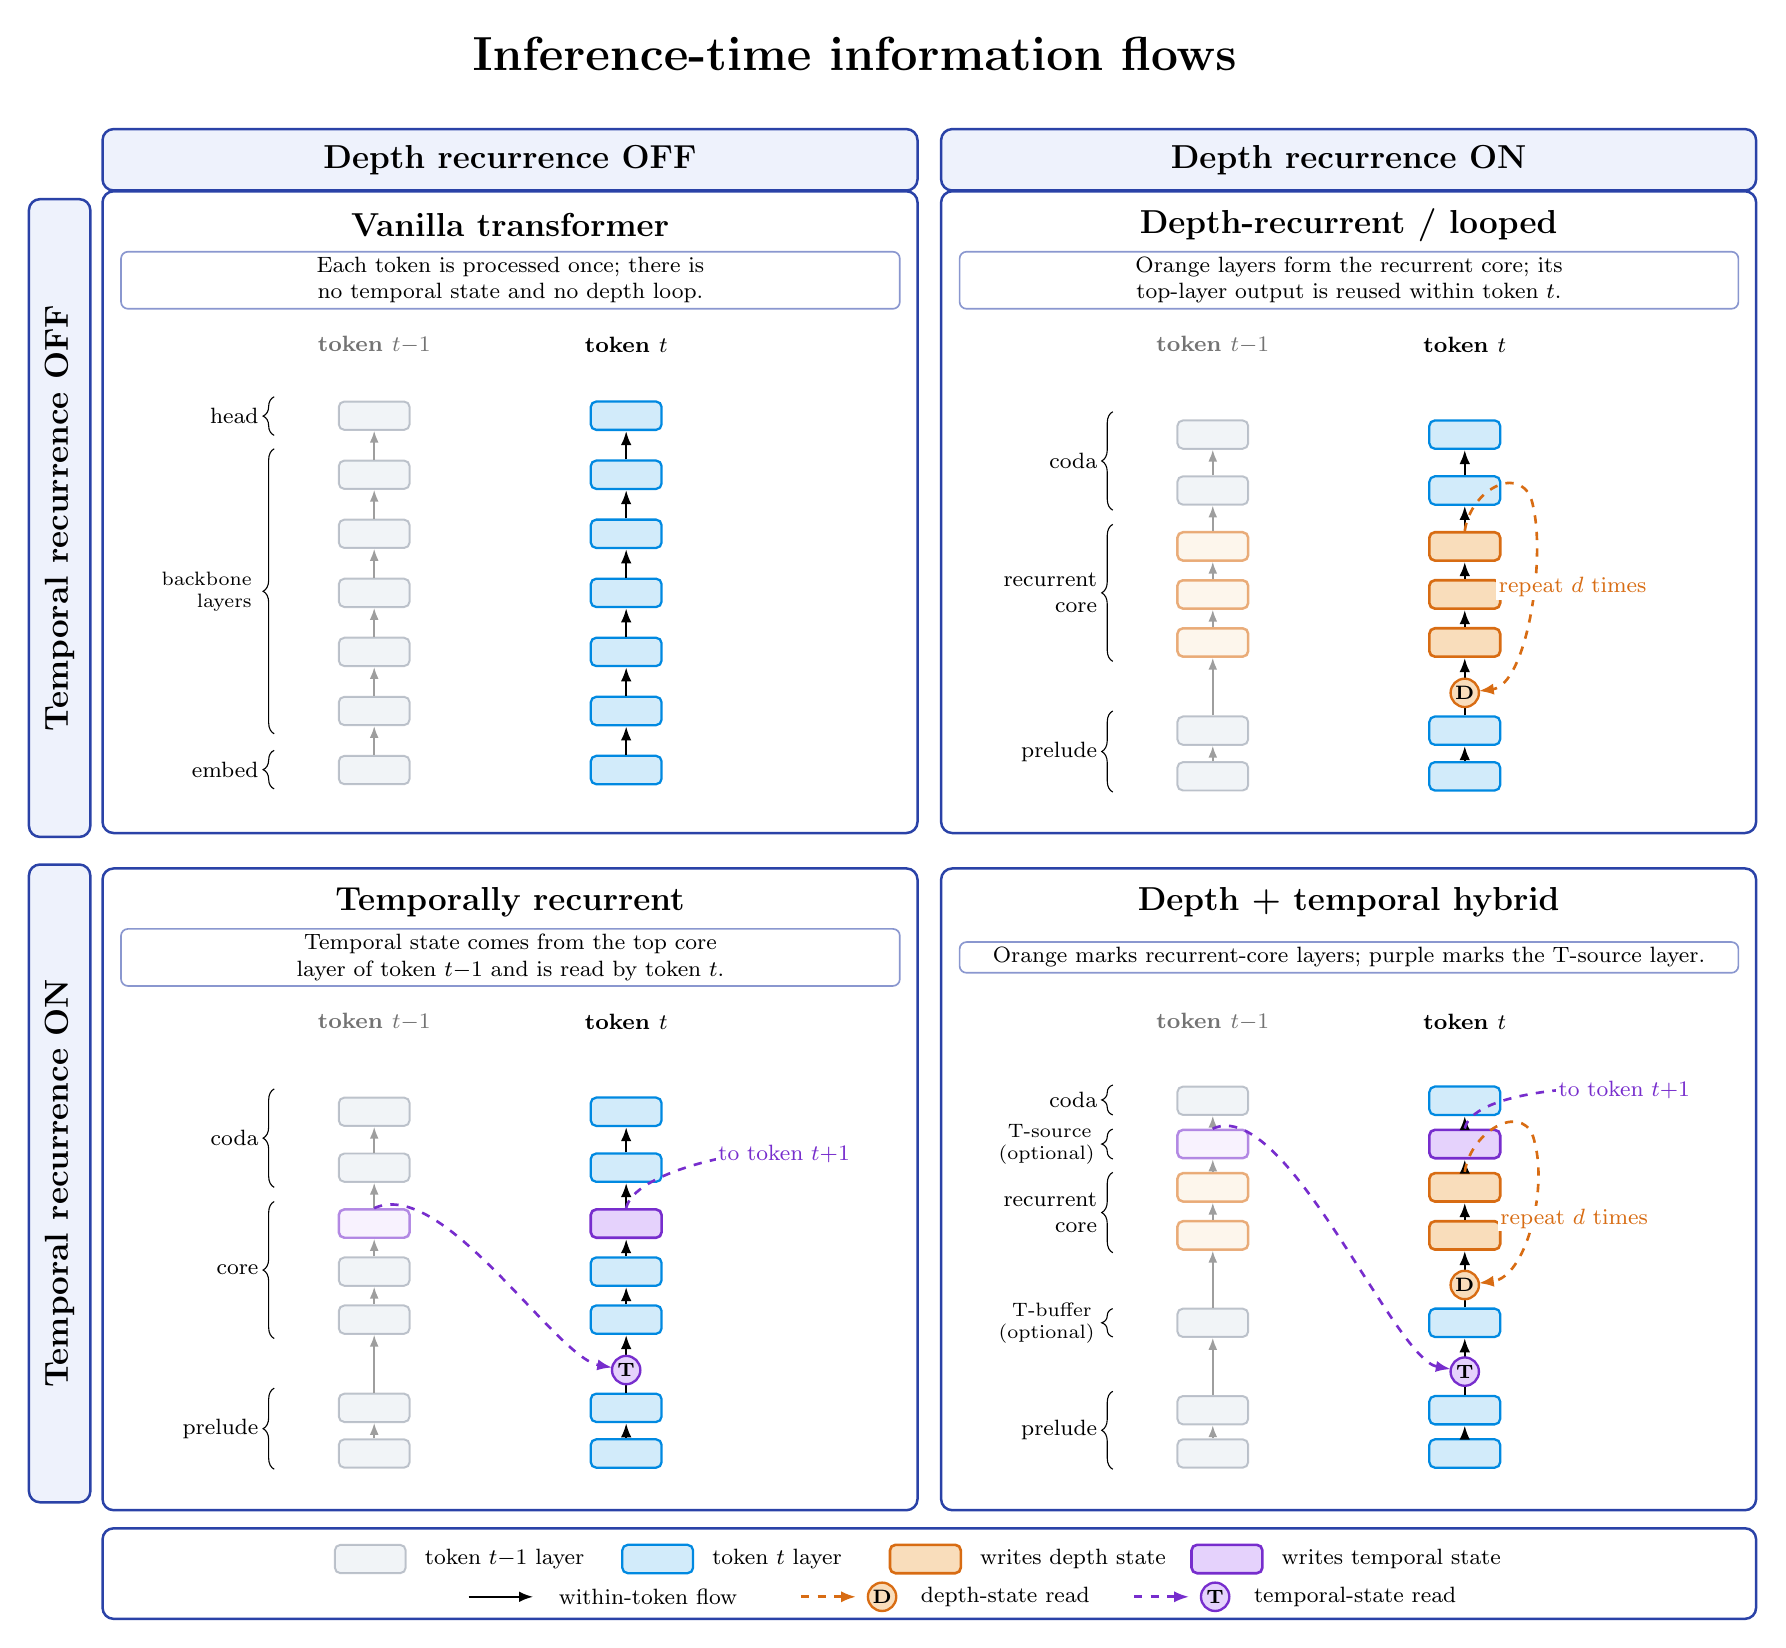
\begin{tikzpicture}[x=1cm,y=1cm]

% ------------------------------------------------------------
% Title and recurrence-axis headers
% ------------------------------------------------------------
\node[font=\bfseries\LARGE] at (11.9,17.45) {Inference-time information flows};

\node[header, minimum width=10.35cm, minimum height=0.78cm, font=\bfseries\large]
  at (7.525,16.10) {Depth recurrence OFF};
\node[header, minimum width=10.35cm, minimum height=0.78cm, font=\bfseries\large]
  at (18.175,16.10) {Depth recurrence ON};

\node[sideheader, minimum width=8.10cm, minimum height=0.78cm, rotate=90, font=\bfseries\large]
  at (1.805,11.55) {Temporal recurrence OFF};
\node[sideheader, minimum width=8.10cm, minimum height=0.78cm, rotate=90, font=\bfseries\large]
  at (1.805,3.10) {Temporal recurrence ON};

% ============================================================
% TOP LEFT -- Vanilla transformer, layer-wise
% ============================================================
\begin{scope}[shift={(2.35,7.55)}]
  \draw[panel] (0,0) rectangle (10.35,8.15);
  \node[font=\bfseries\large] at (5.175,7.72) {Vanilla transformer};
  \node[descbox,text width=9.75cm] at (5.18,7.02)
    {Each token is processed once; there is no temporal state and no depth loop.};

  \node[font=\bfseries\footnotesize,text=black!55] at (3.45,6.20) {token $t{-}1$};
  \node[font=\bfseries\footnotesize] at (6.65,6.20) {token $t$};

  \draw[decorate,decoration={brace,amplitude=4pt}] (2.18,5.05) -- (2.18,5.54)
    node[brace label] {head};
  \draw[decorate,decoration={brace,amplitude=4pt}] (2.18,1.26) -- (2.18,4.88)
    node[brace label,font=\scriptsize,text width=1.15cm] {backbone\\layers};
  \draw[decorate,decoration={brace,amplitude=4pt}] (2.18,0.56) -- (2.18,1.05)
    node[brace label] {embed};

  \foreach \I/\Y in {1/0.80,2/1.55,3/2.30,4/3.05,5/3.80,6/4.55,7/5.30}{
    \node[ghost]  (vg-\I) at (3.45,\Y) {};
    \node[active] (va-\I) at (6.65,\Y) {};
  }
  \foreach \A/\B in {1/2,2/3,3/4,4/5,5/6,6/7}{
    \draw[ghostflow] (vg-\A.north)--(vg-\B.south);
    \draw[flow] (va-\A.north)--(va-\B.south);
  }
\end{scope}

% ============================================================
% TOP RIGHT -- Depth recurrent, layer-wise
% ============================================================
\begin{scope}[shift={(13.00,7.55)}]
  \draw[panel] (0,0) rectangle (10.35,8.15);
  \node[font=\bfseries\large] at (5.175,7.72) {Depth-recurrent / looped};
  \node[descbox,text width=9.75cm] at (5.18,7.02)
    {Orange layers form the recurrent core; its top-layer output is reused within token $t$.};

  \node[font=\bfseries\footnotesize,text=black!55] at (3.45,6.20) {token $t{-}1$};
  \node[font=\bfseries\footnotesize] at (6.65,6.20) {token $t$};

  \draw[decorate,decoration={brace,amplitude=4pt}] (2.18,4.10) -- (2.18,5.35)
    node[brace label] {coda};
  \draw[decorate,decoration={brace,amplitude=4pt}] (2.18,2.18) -- (2.18,3.92)
    node[brace label] {recurrent\\core};
  \draw[decorate,decoration={brace,amplitude=4pt}] (2.18,0.52) -- (2.18,1.55)
    node[brace label] {prelude};

  % token t-1
  \node[ghost]      (dg-1) at (3.45,0.72) {};
  \node[ghost]      (dg-2) at (3.45,1.30) {};
  \node[ghostdepth] (dg-3) at (3.45,2.42) {};
  \node[ghostdepth] (dg-4) at (3.45,3.03) {};
  \node[ghostdepth] (dg-5) at (3.45,3.64) {};
  \node[ghost]      (dg-6) at (3.45,4.35) {};
  \node[ghost]      (dg-7) at (3.45,5.06) {};
  \foreach \A/\B in {1/2,2/3,3/4,4/5,5/6,6/7}{\draw[ghostflow] (dg-\A.north)--(dg-\B.south);}

  % token t
  \node[active]    (da-1) at (6.65,0.72) {};
  \node[active]    (da-2) at (6.65,1.30) {};
  \node[depthmark] (da-3) at (6.65,2.42) {};
  \node[depthmark] (da-4) at (6.65,3.03) {};
  \node[depthmark] (da-5) at (6.65,3.64) {};
  \node[active]    (da-6) at (6.65,4.35) {};
  \node[active]    (da-7) at (6.65,5.06) {};
  \foreach \A/\B in {1/2,2/3,3/4,4/5,5/6,6/7}{\draw[flow] (da-\A.north)--(da-\B.south);}

  \coordinate (dDpos) at (6.65,1.78);
  % Smooth outer loop: top-layer output of recurrent core -> D site.
  \draw[dread,shorten >=1.8mm]
    (da-5.north)
      .. controls +(0.08,0.56) and +(-0.10,0.58) .. (7.52,4.14)
      .. controls +(0.16,-0.70) and +(0.78,0.10) .. (dDpos);
  \node[font=\footnotesize,text=depthdraw,fill=white,inner sep=1pt] at (8.02,3.12) {repeat $d$ times};
  % Draw injection marker after all lines so it sits on top of within-token flow.
  \node[injectD] at (dDpos) {D};
\end{scope}

% ============================================================
% BOTTOM LEFT -- Temporal only, layer-wise
% ============================================================
\begin{scope}[shift={(2.35,-1.05)}]
  \draw[panel] (0,0) rectangle (10.35,8.15);
  \node[font=\bfseries\large] at (5.175,7.72) {Temporally recurrent};
  \node[descbox,text width=9.75cm] at (5.18,7.02)
    {Temporal state comes from the top core layer of token $t{-}1$ and is read by token $t$.};

  \node[font=\bfseries\footnotesize,text=black!55] at (3.45,6.20) {token $t{-}1$};
  \node[font=\bfseries\footnotesize] at (6.65,6.20) {token $t$};

  \draw[decorate,decoration={brace,amplitude=4pt}] (2.18,4.10) -- (2.18,5.35)
    node[brace label] {coda};
  \draw[decorate,decoration={brace,amplitude=4pt}] (2.18,2.18) -- (2.18,3.92)
    node[brace label] {core};
  \draw[decorate,decoration={brace,amplitude=4pt}] (2.18,0.52) -- (2.18,1.55)
    node[brace label] {prelude};

  % token t-1
  \node[ghost]     (tg-1) at (3.45,0.72) {};
  \node[ghost]     (tg-2) at (3.45,1.30) {};
  \node[ghost]     (tg-3) at (3.45,2.42) {};
  \node[ghost]     (tg-4) at (3.45,3.03) {};
  \node[ghosttemp] (tg-5) at (3.45,3.64) {};
  \node[ghost]     (tg-6) at (3.45,4.35) {};
  \node[ghost]     (tg-7) at (3.45,5.06) {};
  \foreach \A/\B in {1/2,2/3,3/4,4/5,5/6,6/7}{\draw[ghostflow] (tg-\A.north)--(tg-\B.south);}

  % token t
  \node[active]   (ta-1) at (6.65,0.72) {};
  \node[active]   (ta-2) at (6.65,1.30) {};
  \node[active]   (ta-3) at (6.65,2.42) {};
  \node[active]   (ta-4) at (6.65,3.03) {};
  \node[tempmark] (ta-5) at (6.65,3.64) {};
  \node[active]   (ta-6) at (6.65,4.35) {};
  \node[active]   (ta-7) at (6.65,5.06) {};
  \foreach \A/\B in {1/2,2/3,3/4,4/5,5/6,6/7}{\draw[flow] (ta-\A.north)--(ta-\B.south);}

  \coordinate (tTpos) at (6.65,1.78);
  % Temporal state exits from the top of the previous token's source layer.
  \draw[tread,shorten >=1.8mm]
    (tg-5.north)
      .. controls +(0.88,0.40) and +(-0.90,0.16) .. (tTpos);
  % Current token emits state from the same top-core layer to token t+1.
  \draw[tread]
    (ta-5.north)
      .. controls +(0.10,0.46) and +(-0.42,0.04) .. (8.55,4.52);
  \node[anchor=west,font=\footnotesize,text=tempdraw,fill=white,inner sep=1pt] at (7.78,4.53) {to token $t{+}1$};
  \node[injectT] at (tTpos) {T};
\end{scope}

% ============================================================
% BOTTOM RIGHT -- Hybrid, layer-wise
% ============================================================
\begin{scope}[shift={(13.00,-1.05)}]
  \draw[panel] (0,0) rectangle (10.35,8.15);
  \node[font=\bfseries\large] at (5.175,7.72) {Depth + temporal hybrid};
  \node[descbox,text width=9.75cm] at (5.18,7.02)
    {Orange marks recurrent-core layers; purple marks the T-source layer.};

  \node[font=\bfseries\footnotesize,text=black!55] at (3.45,6.20) {token $t{-}1$};
  \node[font=\bfseries\footnotesize] at (6.65,6.20) {token $t$};

  \draw[decorate,decoration={brace,amplitude=4pt}] (2.18,5.02) -- (2.18,5.40)
    node[brace label] {coda};
  \draw[decorate,decoration={brace,amplitude=4pt}] (2.18,4.46) -- (2.18,4.84)
    node[brace label,font=\scriptsize,text width=1.18cm] {T-source\\(optional)};
  \draw[decorate,decoration={brace,amplitude=4pt}] (2.18,3.27) -- (2.18,4.29)
    node[brace label] {recurrent\\core};
  \draw[decorate,decoration={brace,amplitude=4pt}] (2.18,2.20) -- (2.18,2.56)
    node[brace label,font=\scriptsize,text width=1.18cm] {T-buffer\\(optional)};
  \draw[decorate,decoration={brace,amplitude=4pt}] (2.18,0.52) -- (2.18,1.51)
    node[brace label] {prelude};

  % token t-1
  \node[ghost]      (hg-1) at (3.45,0.72) {};
  \node[ghost]      (hg-2) at (3.45,1.27) {};
  \node[ghost]      (hg-3) at (3.45,2.38) {};
  \node[ghostdepth] (hg-4) at (3.45,3.49) {};
  \node[ghostdepth] (hg-5) at (3.45,4.10) {};
  \node[ghosttemp]  (hg-6) at (3.45,4.65) {};
  \node[ghost]      (hg-7) at (3.45,5.20) {};
  \foreach \A/\B in {1/2,2/3,3/4,4/5,5/6,6/7}{\draw[ghostflow] (hg-\A.north)--(hg-\B.south);}

  % token t
  \node[active]    (ha-1) at (6.65,0.72) {};
  \node[active]    (ha-2) at (6.65,1.27) {};
  \node[active]    (ha-3) at (6.65,2.38) {};
  \node[depthmark] (ha-4) at (6.65,3.49) {};
  \node[depthmark] (ha-5) at (6.65,4.10) {};
  \node[tempmark]  (ha-6) at (6.65,4.65) {};
  \node[active]    (ha-7) at (6.65,5.20) {};
  \foreach \A/\B in {1/2,2/3,3/4,4/5,5/6,6/7}{\draw[flow] (ha-\A.north)--(ha-\B.south);}

  \coordinate (hTpos) at (6.65,1.76);
  \coordinate (hDpos) at (6.65,2.86);

  % Temporal feedback from top of previous token's T-source layer.
  \draw[tread,shorten >=1.8mm]
    (hg-6.north)
      .. controls +(0.92,0.42) and +(-0.90,0.16) .. (hTpos);

  % Smooth depth loop from top of the last recurrent-core layer.
  \draw[dread,shorten >=1.8mm]
    (ha-5.north)
      .. controls +(0.08,0.54) and +(-0.10,0.56) .. (7.54,4.66)
      .. controls +(0.16,-0.60) and +(0.78,0.10) .. (hDpos);
  \node[font=\footnotesize,text=depthdraw,fill=white,inner sep=1pt] at (8.04,3.70) {repeat $d$ times};

  % Current token emits temporal state from top of T-source.
  \draw[tread]
    (ha-6.north)
      .. controls +(0.10,0.46) and +(-0.42,0.04) .. (8.58,5.34);
  \node[anchor=west,font=\footnotesize,text=tempdraw,fill=white,inner sep=1pt] at (7.80,5.34) {to token $t{+}1$};

  % Injection circles are drawn last so black within-token flow passes underneath them.
  \node[injectT] at (hTpos) {T};
  \node[injectD] at (hDpos) {D};
\end{scope}

% ------------------------------------------------------------
% Legend
% ------------------------------------------------------------
\begin{scope}[shift={(2.35,-2.43)}]
  \draw[panel] (0,0) rectangle (21.00,1.15);

  \begin{scope}[xshift=2.85cm]
    \node[ghost] at (0.55,0.76) {};
    \node[anchor=west,font=\footnotesize] at (1.12,0.76) {token $t{-}1$ layer};
    \node[active] at (4.20,0.76) {};
    \node[anchor=west,font=\footnotesize] at (4.77,0.76) {token $t$ layer};
    \node[depthmark] at (7.60,0.76) {};
    \node[anchor=west,font=\footnotesize] at (8.17,0.76) {writes depth state};
    \node[tempmark] at (11.43,0.76) {};
    \node[anchor=west,font=\footnotesize] at (12.00,0.76) {writes temporal state};
  \end{scope}

  \begin{scope}[xshift=4.35cm]
    \draw[flow] (0.30,0.28) -- (1.12,0.28);
    \node[anchor=west,font=\footnotesize] at (1.32,0.28) {within-token flow};

    \draw[dread] (4.52,0.28) -- (5.22,0.28);
    \node[injectD] at (5.55,0.28) {D};
    \node[anchor=west,font=\footnotesize] at (5.92,0.28) {depth-state read};

    \draw[tread] (8.75,0.28) -- (9.45,0.28);
    \node[injectT] at (9.78,0.28) {T};
    \node[anchor=west,font=\footnotesize] at (10.15,0.28) {temporal-state read};
  \end{scope}
\end{scope}

\end{tikzpicture}
\end{document}
